\chapter{Исследовательская часть}

\section{Технические характеристики}

Технические характеристики устройства, на котором выполнялось тестирование:

\begin{itemize}
	\item Операционная система: Manjaro \cite{manjaro} Linux x86\_64.
	\item Память: 8 GiB.
	\item Процессор: Intel® Core™ i5-8265U\cite{intel}.
\end{itemize}

Тестирование проводилось на ноутбуке, включенном в сеть электропитания. Во
время тестирования ноутбук был нагружен только встроенными приложениями
окружения, окружением, а также непосредственно системой тестирования.

\section{Примеры работы программы}

В данном подразделе представлены примеры работы программы. На рисунке
\ref{img:rus} приведен пример работы программы при вводе строк в русской
раскладке и равными расстояниями Левенштейна и Дамерау-Левенштейна. На рисунке
\ref{img:eng} приведен пример работы программы при вводе строк в английской
раскладке и разными полученными значениями расстояний.

\begin{figure}[ht!]
\begin{center}
    \begin{minipage}[h]{0.4\linewidth}
        \begin{center}
            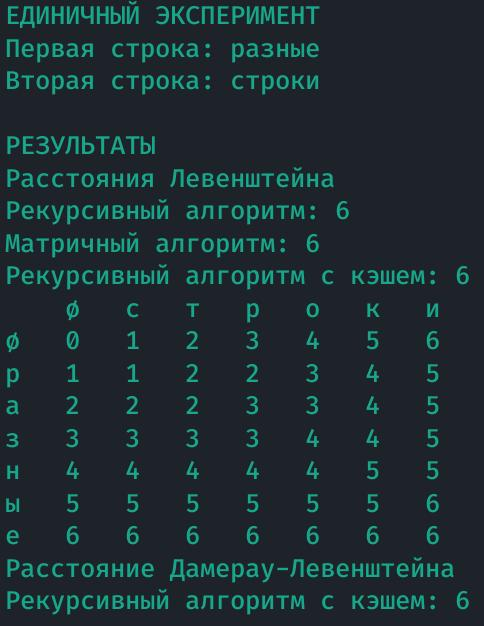
\includegraphics[height=6.5cm]{../data/img/exRus.jpg}
            \caption{Пример работы программы в русской раскладке}
            \label{img:rus}
        \end{center}
    \end{minipage}
    \hspace{2ex}
    \begin{minipage}[h]{0.4\linewidth}
        \begin{center}
            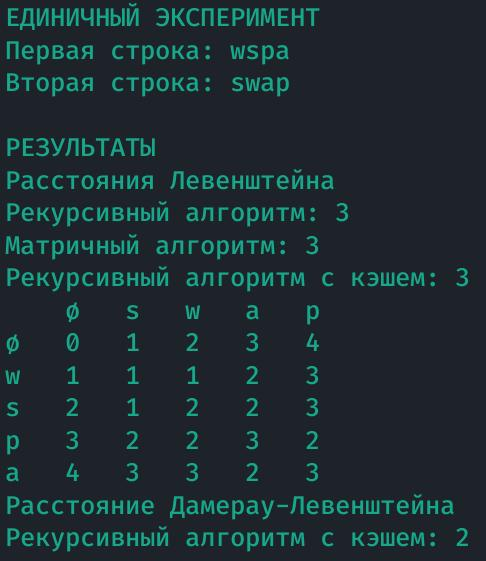
\includegraphics[height=6.5cm]{../data/img/exEng.jpg}
            \caption{Пример работы программы в английской раскладке}
            \label{img:eng}
        \end{center}
    \end{minipage}
\end{center}
\end{figure}

\section{Результаты тестирования}

В таблице \ref{tab:testRes} приведены результаты работы программы на тестах,
описанных в таблице \ref{tab:tests}. В результате сравнения ожидаемого и
полученного результата делаем вывод, что все тесты были пройдены.

\begin{table}[h]
	\begin{center}
		\caption{\label{tab:testRes}Результаты тестирования}
		\begin{tabular}{|c|c|c|c|}
			\hline
			& & \multicolumn{2}{c|}{\bfseries Полученный результат}\\ \cline{3-4}
			\bfseries Строка 1  & \bfseries Строка 2 &
            \bfseries Левенштейн & \bfseries Дамерау-Левенштейн
			\csvreader{../data/csv/tests.csv}{}
			{\\\hline \csvcoli&\csvcolii&\csvcoliii&\csvcoliv}
			\\\hline
		\end{tabular}
	\end{center}
\end{table}

\section[Постановка эксперимента по замеру времени]
        {Постановка ~~эксперимента ~~по ~~замеру времени}

Был проведен эксперимент для определения влияния длины строк на время работы
каждого вида алгоритмов и выявления более эффективной по времени реализации.
Тестирование проводилось на строках длиной от 10 до 170 с шагом 20. Так
как от запуска к запуску процессорное время, затрачиваемое на выполнение
агоритма менялось в определенном промежутке времени, необходимо было усреднить
вычисляемые значения. Для этого алгоритм на каждом значении длины строк
запускался 10 раз, и для полученных 10 значений определялось среднее
арифметическое, которое и заносилось в таблицу результатов.

Так как алгоритмы поиска расстояния Левенштейна и Дамерау"=Левенштейна
подобны друг другу не имело особого практического значения делать замеры
для каждого из алгоритмов, поэтому были проведены замеры времени для различных
реализации поиска расстояния Левенштейна, а также для реализации с кэшем
каждого из алгоритмов. Таким образом, были получены экспериментальные значения
для сравнения разный реализаций одного алгоритма и сравнения одинаковых
реализаций разных алгоритмов.

\section{Результаты эксперимента}

В таблице \ref{tab:cmpLev} представлены результаты измерения времени для
разных реализаций алгоритма поиска расстояния Левенштейна. Так как даже при
длине в 10 символов рекурсивный алгоритм работал в 20-50 тысяч раз медленнее
реализаций с матрицей, вычисления при больших длинах не производились, что
помечено в таблице как $None$. На основе табличных данных построены графики
зависимости времени работы каждой из реализаций с использованием матрицы от
длины строк \ref{img:cmpLev}.
\begin{table}[h]
	\begin{center}
		\caption{\label{tab:cmpLev}Время работы различных реализаций
                алгоритма поиска расстояния Левенштейна (время в наносекундах)}
		\begin{tabular}{|c|c|c|c|}
			\hline
			\bfseries Длина  & \bfseries Рекурсивный &
            \bfseries Матричный & \bfseries Рекурсивный с кэшем 
			\csvreader{../data/csv/cmpLev.csv}{}
			{\\\hline \csvcoli&\csvcolii&\csvcoliii&\csvcoliv}
			\\\hline
		\end{tabular}
	\end{center}
\end{table}
\noindent
\img{5cm}{cmpLevNT}{Графики зависимости времени выполнения алгоримтов
                    поиска расстояния Левенштейна от длины строк}{cmpLev}

В таблице \ref{tab:LvsDL} представлены результаты измерения времени для
реализации с кэшем алгоримтов поиска расстояний Левенштейна и
Дамерау-Левенштейна. На основе табличных данных построены графики зависимости
времени работы каждого алгоритма от длины строк \ref{img:LvsDL}.

\begin{table}[h]
	\begin{center}
		\caption{\label{tab:LvsDL}Время работы алгоритмов с кэшем поиск
                 расстояния Левенштейна и Дамерау-Левенштейна}
		\begin{tabular}{|c|c|c|c|}
			\hline
			\bfseries Длина  & \bfseries Левенштейн &
            \bfseries Дамерау-Левенштейн
			\csvreader{../data/csv/LvsDL.csv}{}
			{\\\hline \csvcoli&\csvcolii&\csvcoliii}
			\\\hline
		\end{tabular}
	\end{center}
\end{table}
\clearpage
\noindent
\img{5cm}{LvsDLNT}{Графики зависимости времени выполнения алгоритмов с кэшем
                   поиска расстояния Левенштейна и Дамерау-Левенштейна
                   от длины строк}{LvsDL}

\section{Вывод}

Рекурсивный алгоритм поиска расстояния Левенштейна работает в 20-50 тысяч раз
дольше алгоритмов, использующих матрицу, уже при значении длин строк, равных
10, что свидельствует о неэффективности этого алгоритма по времени. Матричный
алгоритм и алгоритм с кэшем работают в порядки раз быстрее рекурсивного
алгоритма. Сравнение данных алгоритмов между друг другом приводит нас к выводу
о том, что на значениях длин строк до 200 матричный алгоритм работает примерно
в 1.9 раз быстрее рекурсивного алгоритма с кэшем.

Разница во времени выполнения рекурсивных алгоритмов с кэшем поиска расстояния
Левенштейна и Дамерау-Левенштейна незначительна, а именно при поиске
расстояния Дамерау-Левенштейна алгоримт работает примерно 1.1 раза дольше,
что объясняется проверкой дополнительной операции, которая в свою очередь
позволяет сократить число операций для исправления частой ошибки при наборе
текста к клавитуры.
